\subsubsection{Materials}
Three scenes was constructed for the test. The first was an environment with simple geometry scene. The second was used in the first part of the test when participants were introduced to the camera tool and had to complete 5 tasks. The third level was for the creative part of the test when participants had to envision the camera movement in an environment and then implement it. 

\begin{figure*}[htbp]
\centering
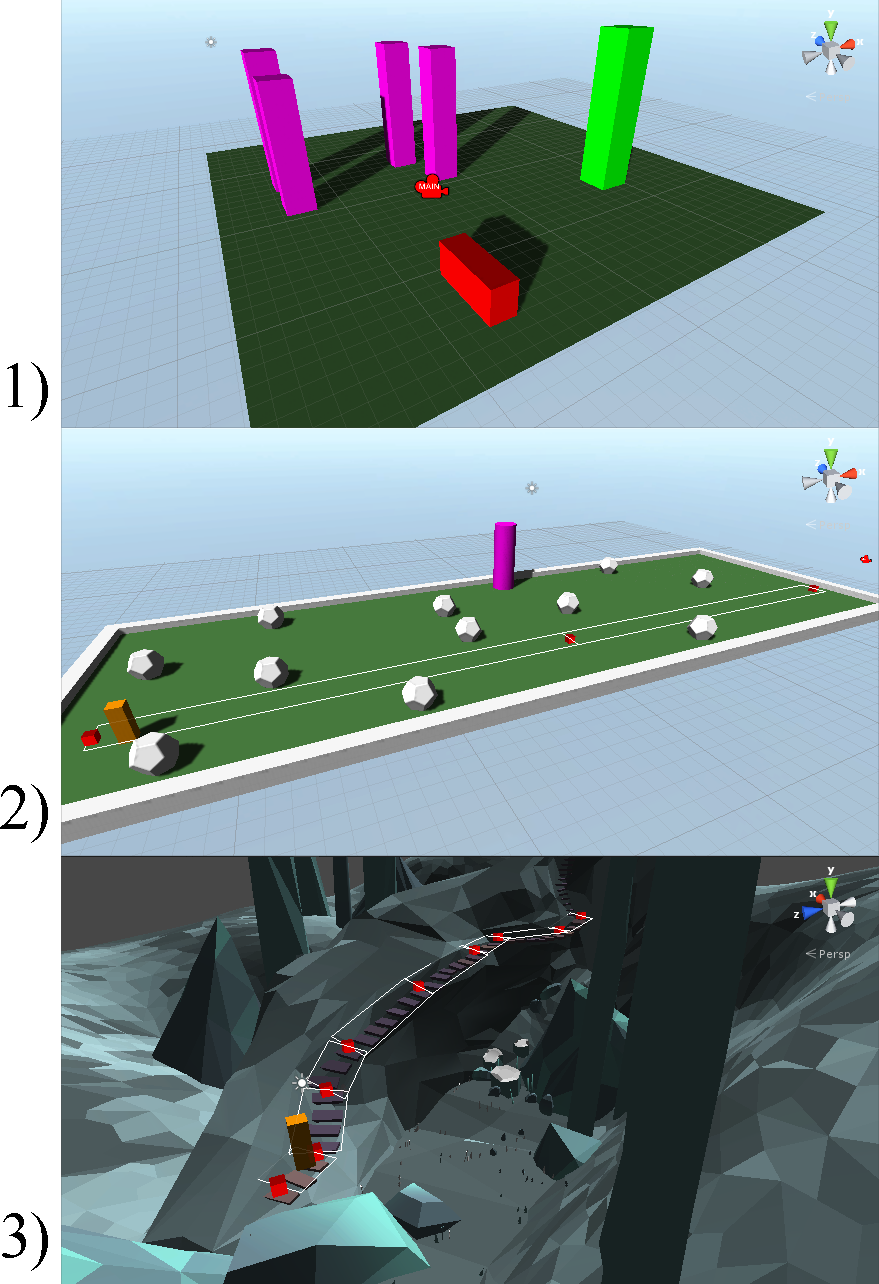
\includegraphics[width=0.45\textwidth]{Pics/sceneAll}
\caption{1) The participant was instructed to move the camera to the top of the green cube, between the purple pillars and to the bottom of the red cube and then rotate the camera to look at the purple pillars. 2) A flat plane with simple geometry to make it easier to see differences when changing camera settings. 3) A mountainous environment with a staircase attached to the mountainside.}
\label{fig:sceneAll}
\end{figure*}